% #############################################################################
% This is Chapter 1
% !TEX root = ../main.tex
% #############################################################################
% Change the Name of the Chapter i the following line
\chapter{Introduction}
% The following line allows to ref this chapter
\label{chap:intro}

The continuous growth and expansion of the world population and the correspondent increase of energy needs, is one of the most relevant topics of the century. The issues caused by the increasing usage of fossil fuels and the amount of carbon dioxide produced everyday is affecting our lives and the future of the planet. In 2019, Industry and buildings account for over 90\% of global electricity demand today, while transport makes up less than 2\% \cite{iea}. Recent studies show that the building sector represents 39\% and 40\% of the energy consumption and 38\% and 36\% of the CO2 emissions in the U.S. \cite{CivilUS} and Europe\cite{CivilEU}, respectively. The expansion of office buildings and the multiplication of the amount of energy needed in order to satisfy the demands of a society that is becoming more and more technologically dependent, are two catalysts for the recent increase of energy consumption. 



On the other hand, sustainable alternatives have also emerged to replace some less ecological social habits. Electric cars are the best example of this. The adoption of electric cars is a practice that has been increasing in the last decade and is expected to grow even more in the next two. Currently the major limitation is the autonomy of the cars, since the batteries still do not have, in most cases, enough capacity to equal the autonomy performance of a fuel car. In this sense, a solution that has been adopted is the installation of charging stations in both residential and office buildings. According to \cite{charger}, the infrastructure for \ac{EV} charging is expanding and in 2019, there were about 7.3 million chargers worldwide, of which about 6.5 million were private. The power spent on charging electric cars in buildings is a new factor to be studied, both in the influence it has on the energy consumption of the building and the reduction of energy waste while using it.


The extent of available data is also multiplying, and the analysis and modeling of this data is becoming essential to minimize energy waste. Modern infrastructures are already equipped with systems able to monitor and control power usage, and there has been an increase in the number of chargers for electric cars installed in garages. The technology also evolved to allow buildings to produce their own energy. The implementation of \ac{PV} panels in buildings is an increasingly common practice. Despite the low efficiencies (from 15\% to 17\% \cite{pv}), \ac{PV} panels are becoming an important energy source for buildings, both  residential and non-residential. 









\section{Problem statement and objectives}


\ac{EDP} is a vertically integrated energy company with a consolidated position in the Iberian Peninsula, both in terms of electricity generation, distribution and supply, and gas supply. The energy consumption of \ac{EDP}'s Lisbon building can be divided into two categories, controlled and uncontrolled consumption. Within the category of uncontrolled consumption, some factors are identified such as the \ac{HVAC} system, lighting, among others. These factors are said to be uncontrolled, as they generally depend directly on factors such as the outside temperature and the occupancy rate of the building, respectively, variables that cannot be controlled. When it comes to controlled consumption, in the building's parking garage there is an electric car charging system for employees, denominated \ac{EVCS}. 

The main functionality of this system is to manage the charging of all the \ac{EV}s connected to the \ac{EVCSs}. This system is able to assign exactly the amount of power supplied to each vehicle, and is able to prioritize the charging, for example, a vehicle that already has 80$\%$ of battery capacity, has less priority than a discharged vehicle that has been recently connected to the grid. The system can also manage the charging procedure based on the instantaneous available power of the building, providing more capacity when there is less overall consumption, and reducing the capacity otherwise. The decision making ability of the \ac{EVCS} makes the charging of \ac{EV}s a controlled consumption process. When it comes to production, unlike generality, the building is equipped with 70 kWp (kilowatt "peak") of solar generation, which means it also has the capacity to generate power. 


%The ability to forecast building power consumption's and the respective power available at each time, can be decisive to optimize power usage in a building.  


%Regarding energy profile, there are two main types of buildings, residential buildings and non-residential buildings. A building should be regarded as residential building when more than half of the floor area is used for dwelling purposes \cite{OECD}. On the other hand, non-residential buildings consists of buildings other than dwellings, including fixtures, facilities and equipment that are integral parts of the structures and costs of site clearance and preparation \cite{OECD}. The work presented focuses on non-residential buildings, more specifically office buildings.


Although this system is already implemented and has access to instant information about the building, the \ac{EVCS} does not have the capacity to compute a projection of production and consumption behaviour of the building in the near future. This capacity would bring numerous advantages, since the knowledge of the future available power to use would allow the optimization of the electric vehicle charging procedure, thus saving energy.

Taking into consideration all the listed factors, the work developed in this thesis contributes directly to minimize the unnecessary power consumption, thus contributing to a more sustainable building. At a global scale, the objective is to assist \ac{EVCS} in the handling of power utilization in the  \ac{EV}'s charging procedure. The system has access to current data, namely the total power available at each instant, but it would be useful to obtain a forecast of the power available in the near future. The knowledge of this value would bring enormous advantages, positively impacting the way \ac{EV} charging is managed. The question then arises: "How can one forecast the power available in a near future, in order to optimize the \ac{EVCS}"? The answer to this question is to create a computing architecture capable of predicting the energy available in the future, while using that forecast to feed the \ac{EVCS}. Specifically, the goal is to define a short-term power availability forecast system to help the \ac{EVCS} to manage power supply for \ac{EVCSs}. In Figure \ref{building}, the reader can observe a schematization of all the work developed during this thesis. 

\begin{figure}[h!]
    \centering
    \begin{center}
    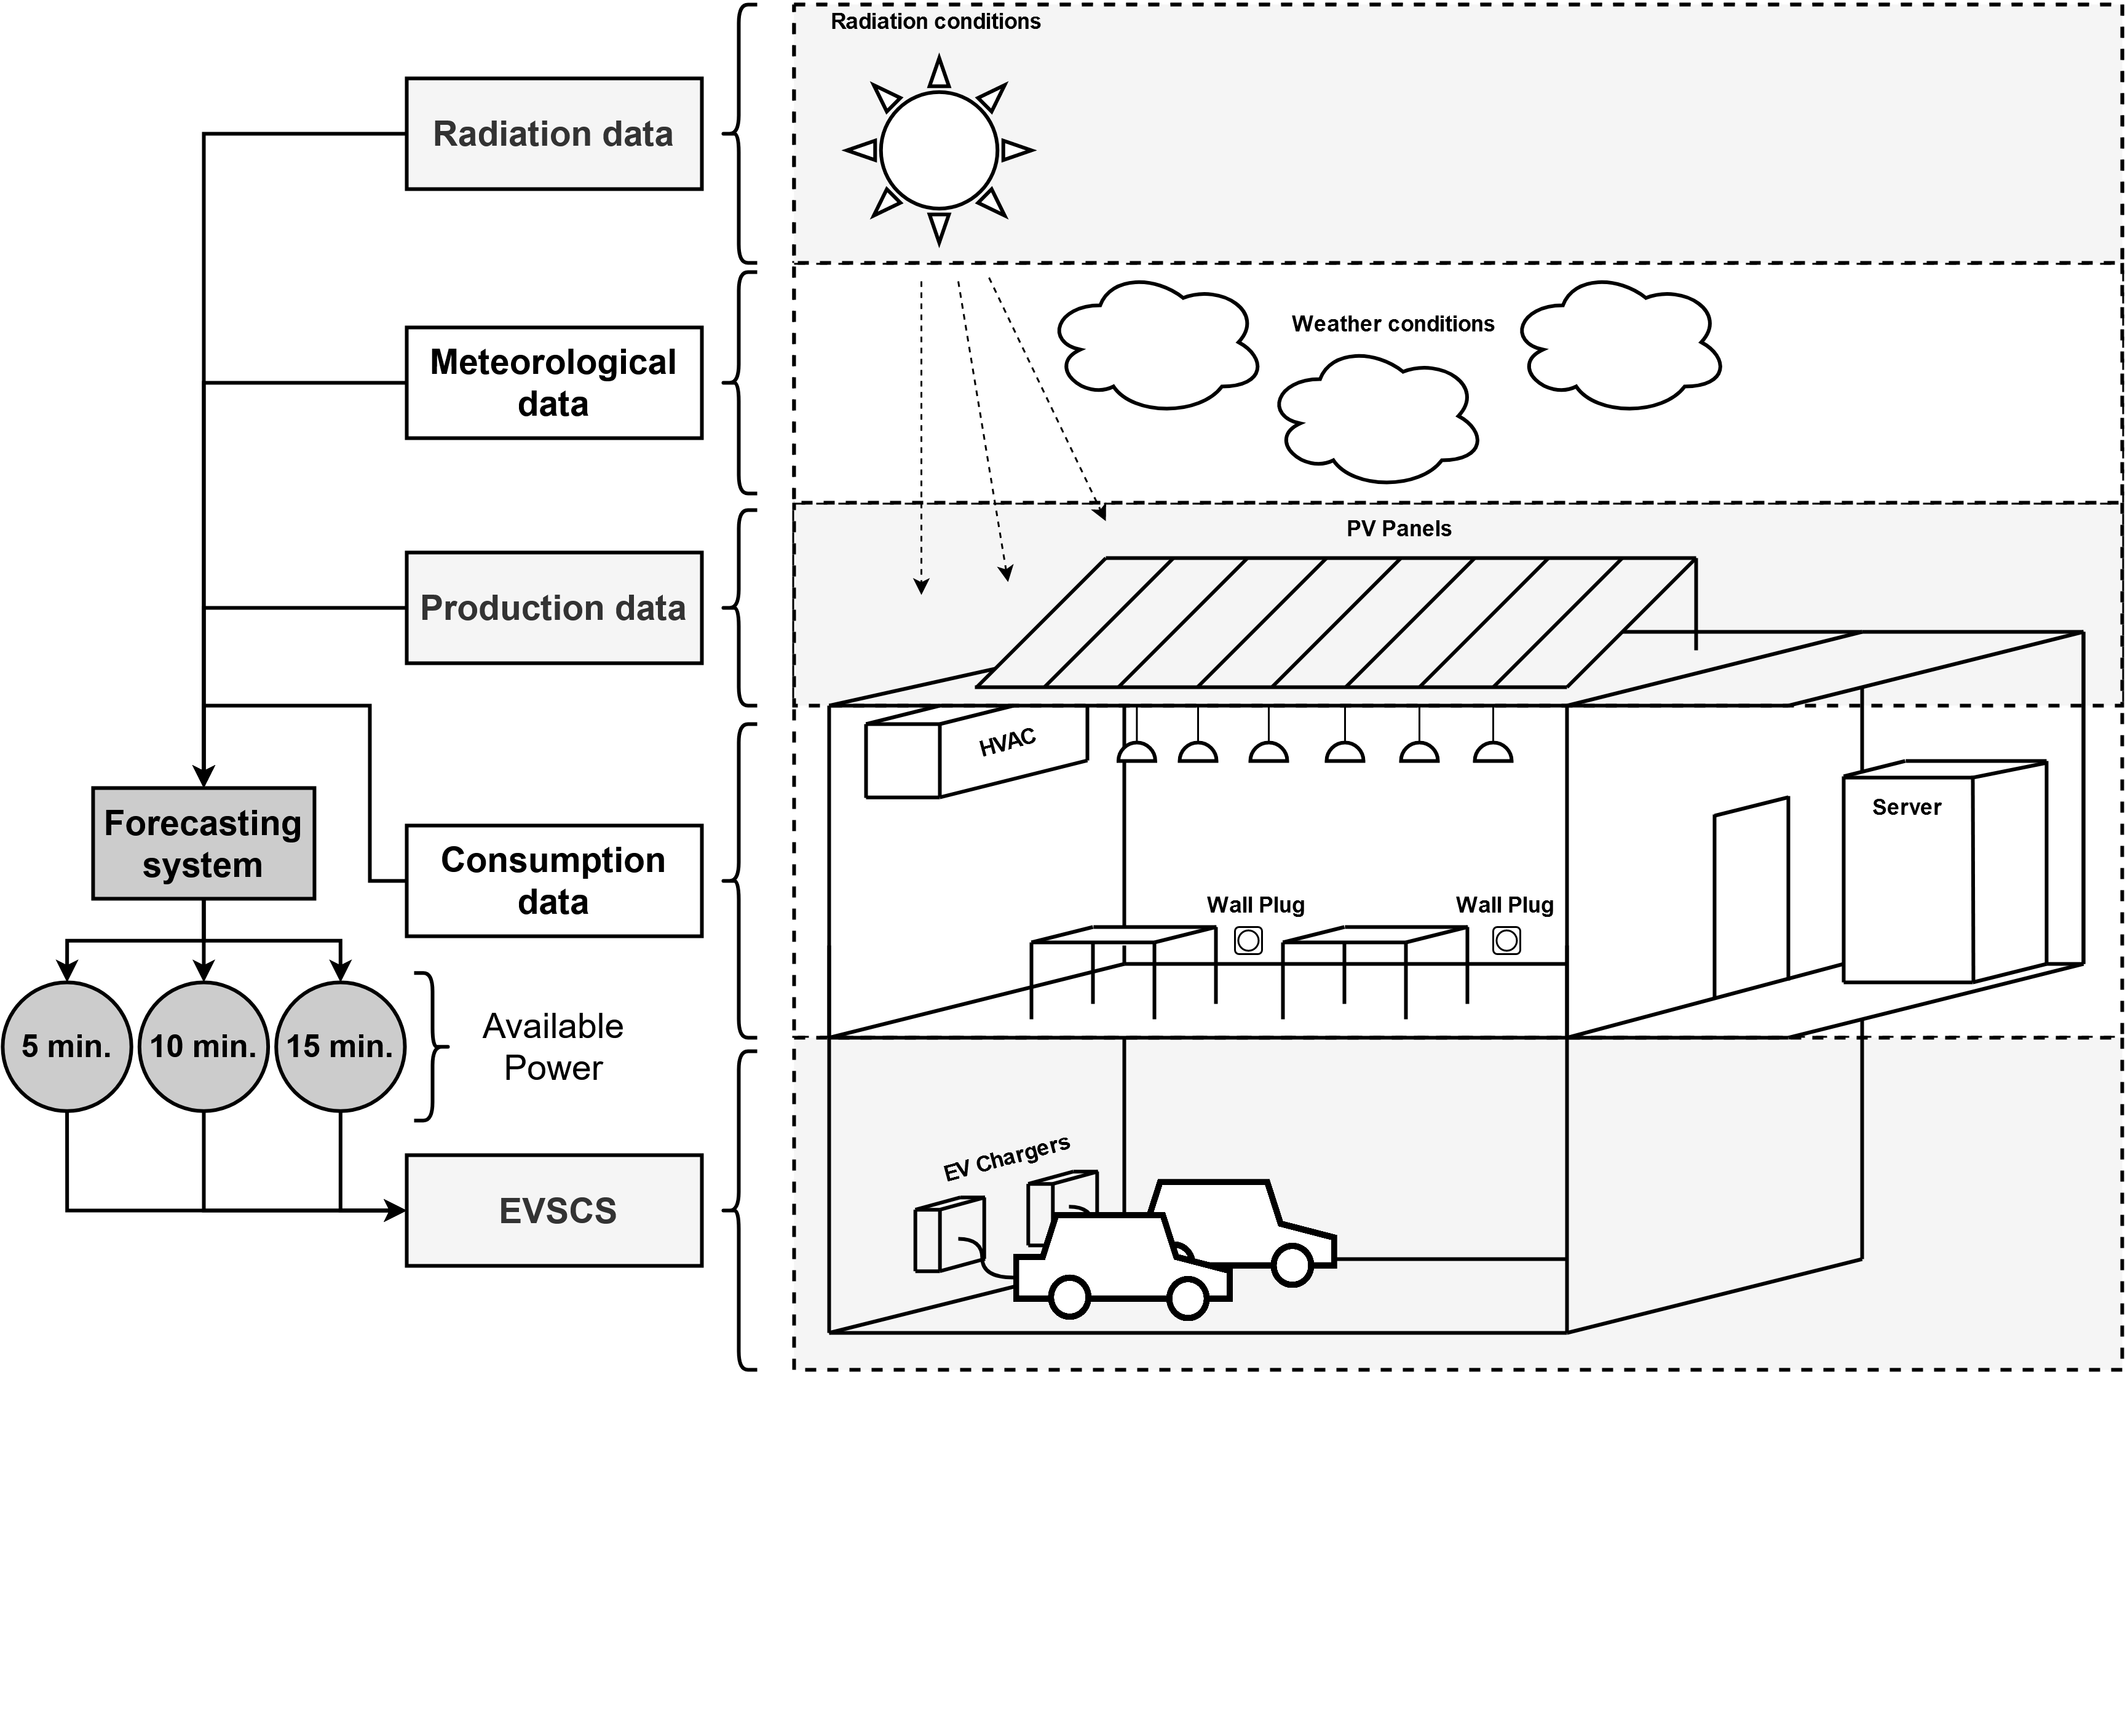
\includegraphics[width=1\textwidth]{Images/BUILDING.png}
    \caption{Building diagram.}
    \label{building}
    \end{center}
\end{figure}

Data from different sources (radiation, meteorology, production and consumption) was used in the construction of a predictive model whose outputs are used as inputs in the \ac{EVCS}. The expected result of the research should be (but not limited to) a maximum and minimum power output forecast algorithm to boost the capabilities of the \ac{EVCS} by predicting \ac{EDP}'s building power availability for the next 5, 10 and 15 minutes.

\section{Thesis outcome}

In the course of this dissertation, a predictive model based on \ac{ML} methodologies was developed, namely using \ac{ANNs}, capable of producing forecasts for the available power with a time target of 5, 10 and 15 minutes in the future, for a building that presents two peculiarities: it has \ac{PV} panels for energy production, and it has an electric car charging system in its parking garage. 

A total of four datesets were used, with information on solar radiation and weather conditions of the area where the building is located, provided by \ac{FCUL}, and information regarding the power consumption and power production of the building, provided by \ac{EDP}. These datasests, besides having different dimensions and granularities, presented temporal gaps. It was then necessary to automate a data treatment process in which, regardless of the state in which the data is introduced in the system, it is treated and prepared to respect the structure that allows it to be used as input to the system. Then the processing starts, where a \ac{ANN} architecture produces forecasts for Available power of the building in 5, 10 and 15 minutes. The result of this thesis is a Hybrid Forecasting System capable of generating short-term forecasts of the available power of the building. The forecasts produced by the forecasting system are later provided to the \ac{EVCS}, that uses this information to optimize its decision process. The optimization process of the charging system is outside the scope of this thesis.

\section{Thesis outline}